% This is the HU Berlin LaTeX template, optimized for R Markdown.

% -------------------------------
% --- PREAMBLE ---
% -------------------------------
\documentclass[a4paper,11pt]{article}

\usepackage{amsmath,amssymb,amsfonts,amsthm}    % Typical maths resource packages
\usepackage{graphicx}                           % Packages to allow inclusion of graphics
\usepackage[authoryear]{natbib}                 % literature reference style
\usepackage[bf]{caption}
\usepackage{textcomp}                           % For single quotes
\usepackage{floatrow}                           % For image and table position
\usepackage{booktabs}                           % For tables
% \usepackage[colorlinks=true]{hyperref}                           
% \usepackage[bottom]{footmisc}                   
\usepackage[bottom, flushmargin]{footmisc}                   % For footnotes
\usepackage[citebordercolor={0 1 0}]{hyperref}                           % For creating hyperlinks in cross references
\usepackage{footnotebackref}
\usepackage{tabularx}
\newcolumntype{C}{>{\centering\arraybackslash}X}
\newcolumntype{L}{>{\raggedright\arraybackslash}X}

% -------------------------------
% --- some layout definitions ---
% -------------------------------

% define topline
\usepackage[automark]{scrlayer-scrpage}
\pagestyle{scrheadings}
\automark{section}
\clearscrheadings
\ohead{\headmark}

% define citation style
\bibliographystyle{ecta}

% define page size, margin size
\setlength{\headheight}{1.1\baselineskip}
\voffset=-2cm
\hoffset=-3cm
\textheight24cm
\textwidth15.5cm
\topmargin1cm
\oddsidemargin3cm
\evensidemargin3cm
\setcounter{secnumdepth}{3}
\setcounter{tocdepth}{3}   
  \usepackage[parfill]{parskip} 

% define line spacing = 1.5
\renewcommand{\baselinestretch}{1.5}

% define position of graphics
\floatsetup[figure]{capposition=top, capbesideposition=left}
\floatsetup[table]{capposition=top, capbesideposition=left}
\floatplacement{figure}{h}
\floatplacement{table}{ht}

% save thesis parameters for later
\newcommand{\thesistype}{Bachelor's Thesis}
\newcommand{\thesisauthor}{Daniel Kuhlen}
\newcommand{\thesisdate}{May 05, 2023}

% define tightlist to work with newer versions of pandoc
\providecommand{\tightlist}{%
  \setlength{\itemsep}{0pt}\setlength{\parskip}{0pt}}

% change spacing
\setlength {\parskip}{1em}

% Additional LaTeX parameters added in the YAML header of index.Rmd

% Added code to define CSLReferences environment
\usepackage{etoolbox}
\newlength{\cslhangindent}
\setlength{\cslhangindent}{1.5em}
\newenvironment{CSLReferences}[2] % #1: entry spacing, #2: hanging-indent width
 {\setlength{\cslhangindent}{#2\parindent}%
  \setlength{\parindent}{0pt}%
  \everypar{\setlength{\hangindent}{\cslhangindent}}\ignorespaces}
 {\par}


% --------------------------------------
% --------------------------------------
% --------------------------------------
% --- the structure the tex document ---
% ---  (this our recommendation) -------
% frontmatter:
%   - titlepage (mandatory),
%   - acknowledgement,
%   - abstract,
%   - table of contents (mandatory),
%   - list of abbreviations (not mandatory),
%   - list of figures (not mandatory),
%   - list of tables  (not mandatory) .
%
% body of the thesis (the structure of the thesis body is not mandatory, but the list of literature is mandatory):
%   - introduction,
%   - methods,
%   - data,
%   - results,
%   - conclusion,
%   - literature (mandatory),
%   - appendix (figures, tables).
%
% last page:
%   - declaration of authorship (mandatory).
% --------------------------------------
% --------------------------------------
% --------------------------------------
\begin{document}
% -------------------------------
% --- frontmatter: Title page ---
% -------------------------------
\thispagestyle{empty}
\begin{center}
  {\Large{\bf Sentiment Analysis of German Parliamentary Candidates' Tweets:
A Longitudinal Study on Electioneering Tone and Post-Election Shifts}} \vspace{0.5cm}

  Bachelor's Thesis submitted \\\vspace{0.5cm}
  to \\\vspace{0.5cm}
  \textbf{Prof.~Dr.~Jochen Müller} \\
  \textbf{Prof.~Dr.~Dont Know} \\\vspace{0.5cm}
  Humboldt-Universität zu Berlin \\
  Institut für Sozialwissenschaften \\
  Innenpolitik der Bundesrepublik Deutschland \\
   \vspace{1cm}

  \includegraphics[width=0.35\textwidth]{HU_Logo_small.png}
  
  by \\\vspace{0.5cm}
  \textbf{Daniel Kuhlen} \\
  (609376) \\
  
  \medskip
  \medskip
  in partial fulfillment of the requirements \\
  for the degree of \\
  \textbf{Bachelor of Arts in Sozialwissenschaften} \\\vspace{0.5cm}
  May 05, 2023
  
\end{center}
% ------------------------------------
% --- frontmatter: Acknowledgement ---
% ------------------------------------
\newpage
\hypertarget{acknowledgements}{%
\section*{Acknowledgements}\label{acknowledgements}}
\addcontentsline{toc}{section}{Acknowledgements}

I want to thank Andreas Küpfer for granting me access to his Twitter API,
which enabled the collection of tweets for this thesis. I also extend my
appreciation to Elias Koch, Linda Naddaf, Luna Strauch, Philipp Kuhlen, Vandross
Alage and Zorbey Özcan for their contributions to the manual coding of the tweets.
\pagestyle{plain}
\pagenumbering{roman}   % define page number in roman style
\setcounter{page}{1}    % start page numbering

% -----------------------------
% --- frontmatter: Abstract ---
% -----------------------------
\newpage
\hypertarget{abstract}{%
\section*{Abstract}\label{abstract}}
\addcontentsline{toc}{section}{Abstract}

In this study, I examine the tone of German parliamentary candidates' tweets before and after an election by employing sentiment dictionaries to analyze a large corpus of tweets spanning a one-year period. The objective is to uncover potential patterns and shifts in political communication on social media platforms during electioneering and post-election engagement. By doing so, I aim to contribute to the growing body of literature on political communication and sentiment analysis. This investigation offers valuable insights for political actors, campaign strategists, and scholars interested in the impact of digital communication on political behavior and public opinion.

% -----------------------------
% --- frontmatter: Contents ---
% -----------------------------
\newpage
\tableofcontents
\clearpage

% ----------------------------------------------------------
% --- frontmatter: List of Abbreviations (not mandatory) ---
% ----------------------------------------------------------
\newpage
\hypertarget{list-of-abbreviations}{%
\section*{List of Abbreviations}\label{list-of-abbreviations}}
\addcontentsline{toc}{section}{List of Abbreviations}
\begin{tabular}{rp{0.2cm}lp{1cm}rp{0.2cm}l}
    API     & &  Application Programming Interface
\end{tabular}
% ----------------------------------------------------
% --- frontmatter: List of Figures (not mandatory) ---
% ----------------------------------------------------
\newpage
\listoffigures
\addcontentsline{toc}{section}{List of Figures}

% ---------------------------------------------------
% --- frontmatter: List of Tables (not mandatory) ---
% ---------------------------------------------------
\newpage
\listoftables
\addcontentsline{toc}{section}{List of Tables}

% -------------------------------
% --- main body of the thesis ---
% -------------------------------
\newpage
\pagestyle{plain}       
\setcounter{page}{1}    % start page numbering anew
\pagenumbering{arabic}  % page numbers in arabic style

\hypertarget{introduction}{%
\section{Introduction}\label{introduction}}

\newpage

\hypertarget{theory}{%
\section{Theory}\label{theory}}

\hypertarget{literature-review}{%
\subsection{Literature Review}\label{literature-review}}

\hypertarget{hypotheses}{%
\subsection{Hypotheses}\label{hypotheses}}

\newpage

\hypertarget{methodology}{%
\section{Methodology}\label{methodology}}

\hypertarget{identification-strategy}{%
\subsection{Identification Strategy}\label{identification-strategy}}

\hypertarget{unit-of-analysis}{%
\subsubsection{Unit of Analysis}\label{unit-of-analysis}}

\hypertarget{treatment-and-outcome}{%
\subsubsection{Treatment and Outcome}\label{treatment-and-outcome}}

\hypertarget{assumptions}{%
\subsubsection{Assumptions}\label{assumptions}}

\newpage

\hypertarget{data}{%
\section{Data}\label{data}}

In order to collect the data for analysis, I first obtained the Twitter handles for all relevant accounts using two hand curated datasets: (\protect\hyperlink{ref-konigEPINetzTwitterPoliticians2022}{König 2022}) and (\protect\hyperlink{ref-saltzerTwitterAccountsCandidates2021}{{``Twitter Accounts of Candidates in the {German} Federal Election 2021 ({GLES})''} 2021}). These datasets not only provide the Twitter handles for candidates, politicians, and parties but also offer valuable metadata, including party affiliation, age, and other relevant information. Then I used the Twitter API to crawl all tweets and retweets posted by the accounts within a one year time frame before and after the election for the 20th German Bundestag (federal parliament) on the September 26, 2021.

As a result the final dataset employed contains 994.575 tweets from from 1.536 candidates and 38 party accounts affiliated with the SPD, CDU, FDP, Linke, Grüne and AfD. A detailed descriptions of the variables is provided in Table \ref{tab:apptable}.

\hypertarget{descriptives}{%
\subsection{Descriptives}\label{descriptives}}

Politicians use Twitter extremely unevenly, and systematic differences between the parties are apparent. Representatives from conservative parties with an older electorate tend to use more \emph{traditional} campaign media strategies, whereas politicians affiliated with progressive parties that attract a younger demographic, tend to utilize \emph{modern} campaign media platforms such as Twitter, Instagram, and TikTok \textbf{(CITATION)}.

This is trend holds true for German politicians as well. As shown in Figure \texttt{\ref{fig:plot-percentage-account}}, 73.5\% Grüne candidates have an account on Twitter, compared to a substantially lower 49.6\% of CDU candidates.
\begin{figure}[H]

{\centering 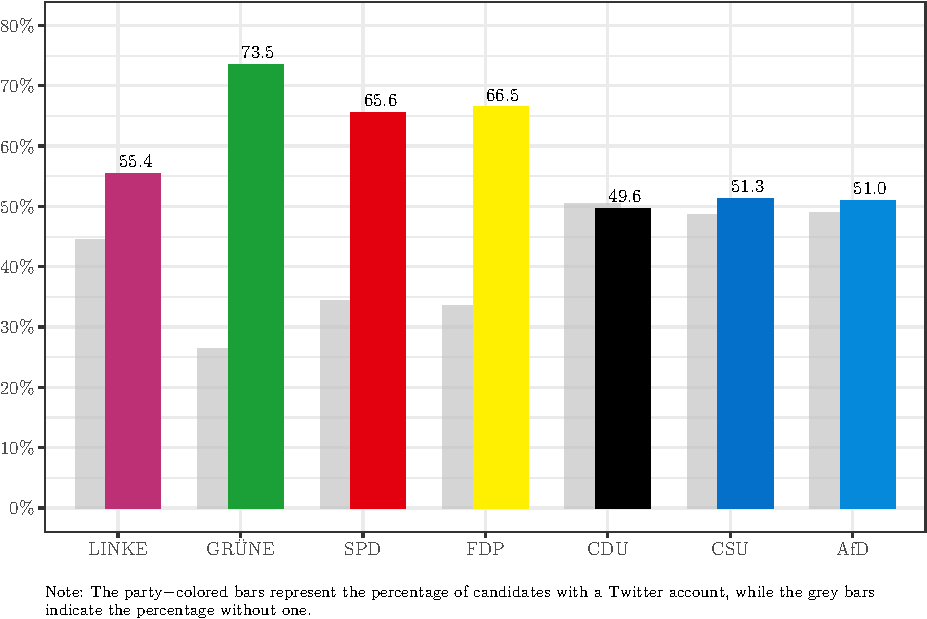
\includegraphics{thesis_files/figure-latex/plot-percentage-account-1} 

}

\caption{Percentage of Candidates with an Account on Twitter}\label{fig:plot-percentage-account}
\end{figure}
\begin{figure}[H]

{\centering 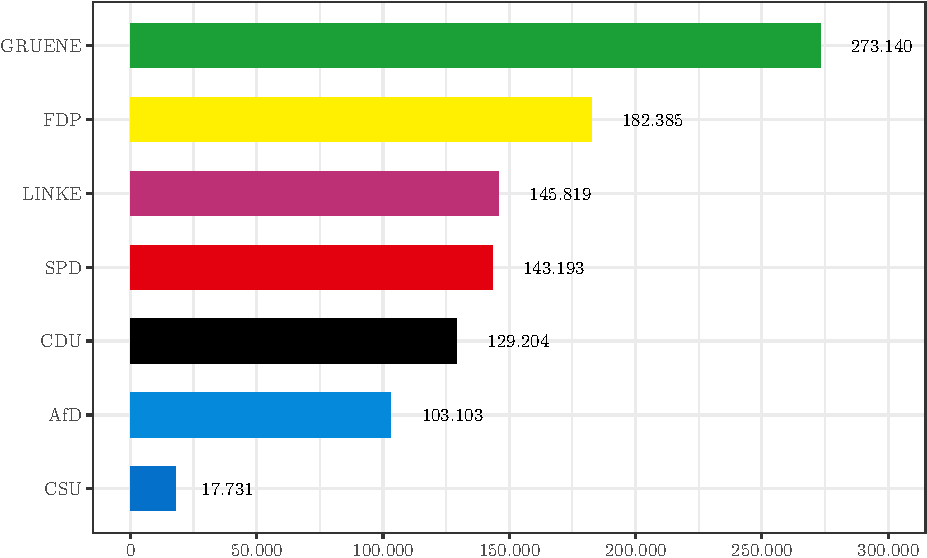
\includegraphics{thesis_files/figure-latex/plot-tweets-amounty-byparty-1} 

}

\caption{Number of Tweets posted by Party}\label{fig:plot-tweets-amounty-byparty}
\end{figure}
\newpage

\hypertarget{results}{%
\section{Results}\label{results}}

\newpage

\hypertarget{conclusion}{%
\section{Conclusion}\label{conclusion}}

\newpage

\hypertarget{references}{%
\section*{References}\label{references}}
\addcontentsline{toc}{section}{References}

\noindent

\setlength{\parindent}{-0.5cm}
\setlength{\leftskip}{0.5cm}
\setlength{\parskip}{8pt}

\hypertarget{refs}{}
\begin{CSLReferences}{1}{0}
\leavevmode\vadjust pre{\hypertarget{ref-konigEPINetzTwitterPoliticians2022}{}}%
König, Tim. 2022. {``{EPINetz Twitter Politicians} 2021.''} {GESIS Data Archive}. \url{https://doi.org/10.7802/2415}.

\leavevmode\vadjust pre{\hypertarget{ref-saltzerTwitterAccountsCandidates2021}{}}%
{``Twitter Accounts of Candidates in the {German} Federal Election 2021 ({GLES}).''} 2021. {GESIS Data Archive}. \url{https://doi.org/10.4232/1.13790}.

\end{CSLReferences}
\indent
\setlength{\parindent}{17pt}
\setlength{\leftskip}{0pt}
\setlength{\parskip}{0pt}

\newpage
\appendix

\hypertarget{appendix}{%
\section{Appendix}\label{appendix}}

\hypertarget{figures}{%
\subsection{Figures}\label{figures}}

\newpage

\hypertarget{tables}{%
\subsection{Tables}\label{tables}}
\begin{table}[H]
    \begin{center}
        \caption{A Detailed Description of the Variables included in the Tweets-Dataset}
        \label{tab:apptable}
        {\footnotesize
        \begin{tabularx}{\textwidth}{L|L|L} % Adjust the column types
        \hline \hline
        Variable Name & Type & Source \\
        \hline
        tweet\_id & Categorical & Twitter API \\
        twitter\_handle & Categorical & Twitter API \\
        text & Text Data & Twitter API \\
        text\_clean & Text Data & Twitter API \\
        language & Categorical & Twitter API \\
        tweet\_date & Date & Twitter API \\
        retweet\_count & Continuous & Twitter API \\
        like\_count & Continuous & Twitter API \\
        quote\_count & Continuous & Twitter API \\
        name & Categorical & GLES / EPIN \\
        gender & Categorical & GLES / EPIN \\
        party & Categorical & GLES / EPIN \\
        district\_name & Categorical & GLES / EPIN \\
        district\_number & Categorical & GLES / EPIN \\
        region & Categorical & GLES / EPIN \\
        incumbent & Binary & GLES \\
        listed\_candidate & Binary & GLES \\
        direct\_candidate & Binary & GLES \\
        binary\_federal\_parliamentarian & Binary & EPIN \\
        binary\_state\_parliamentarian & Binary & EPIN \\
        binary\_european\_parliamentarian & Binary & EPIN \\
        binary\_federal\_state\_secretary & Binary & EPIN \\
        binary\_state\_state\_secretary & Binary & EPIN \\
        binary\_federal\_minister & Binary & EPIN \\
        binary\_state\_minister & Binary & EPIN \\
        user\_verified & Binary & Twitter API \\
        user\_location & Categorical & Twitter API \\
        user\_created\_at & Date & Twitter API \\
        user\_url & Categorical & Twitter API \\
        user\_tweet\_count & Continuous & Twitter API \\
        user\_list\_count & Continuous & Twitter API \\
        user\_followers\_count & Continuous & Twitter API \\
        user\_following\_count & Continuous & Twitter API \\
        \hline \hline
        \end{tabularx}}
    \end{center}
\end{table}
% change rmd_files in `_bookdown.yml` files to determine order
% note that references and appendix are also contained here.

% --------------------------------------------
% --- last page: Declaration of Authorship ---
% --------------------------------------------

\newpage
\thispagestyle{empty}
\hypertarget{declaration-of-authorship}{%
\section*{Declaration of Authorship}\label{declaration-of-authorship}}

I hereby confirm that I have authored this \thesistype{} independently and
without use of others than the indicated sources. All passages which are
literally or in general matter taken out of publications or other sources are
marked as such.
\vspace{1cm}

Berlin, \thesisdate{}
\vspace{3cm}

. . . . . . . . . . . . . . . . . . . . . . . . . . . . . . .
\vspace{0.1cm}

\thesisauthor{}


\end{document}
